\section{Webapp-Sandbox}\label{sec:nutzung-uber-webapp}

Zur interaktiven Nutzung der Klassifizierung wurde eine \emph{Sandbox} in Form einer Webapp entwickelt. Sie verbindet einen vollwertigen \ac{BPMN}-Editor auf Basis von \texttt{BPMN.js} \cite{bpmn-js} mit der in Kapitel~\ref{sec:api-design} beschriebenen HTTP-Schnittstelle und macht die Analyse damit intuitiv bedienbar. In der Sandbox können \ac{BPMN}-Modelle erstellt, verändert, exportiert und importiert, sowie auf Datenschutzrelevanz analysiert werden. Als kritisch klassifizierte Aktivitäten werden nach der Analyse direkt im Editor farblich hervorgehoben, wie in Abbildung \ref{fig:sandbox-frontend-analyzed-model} zu sehen ist.

\begin{figure}[h]
    \centering
    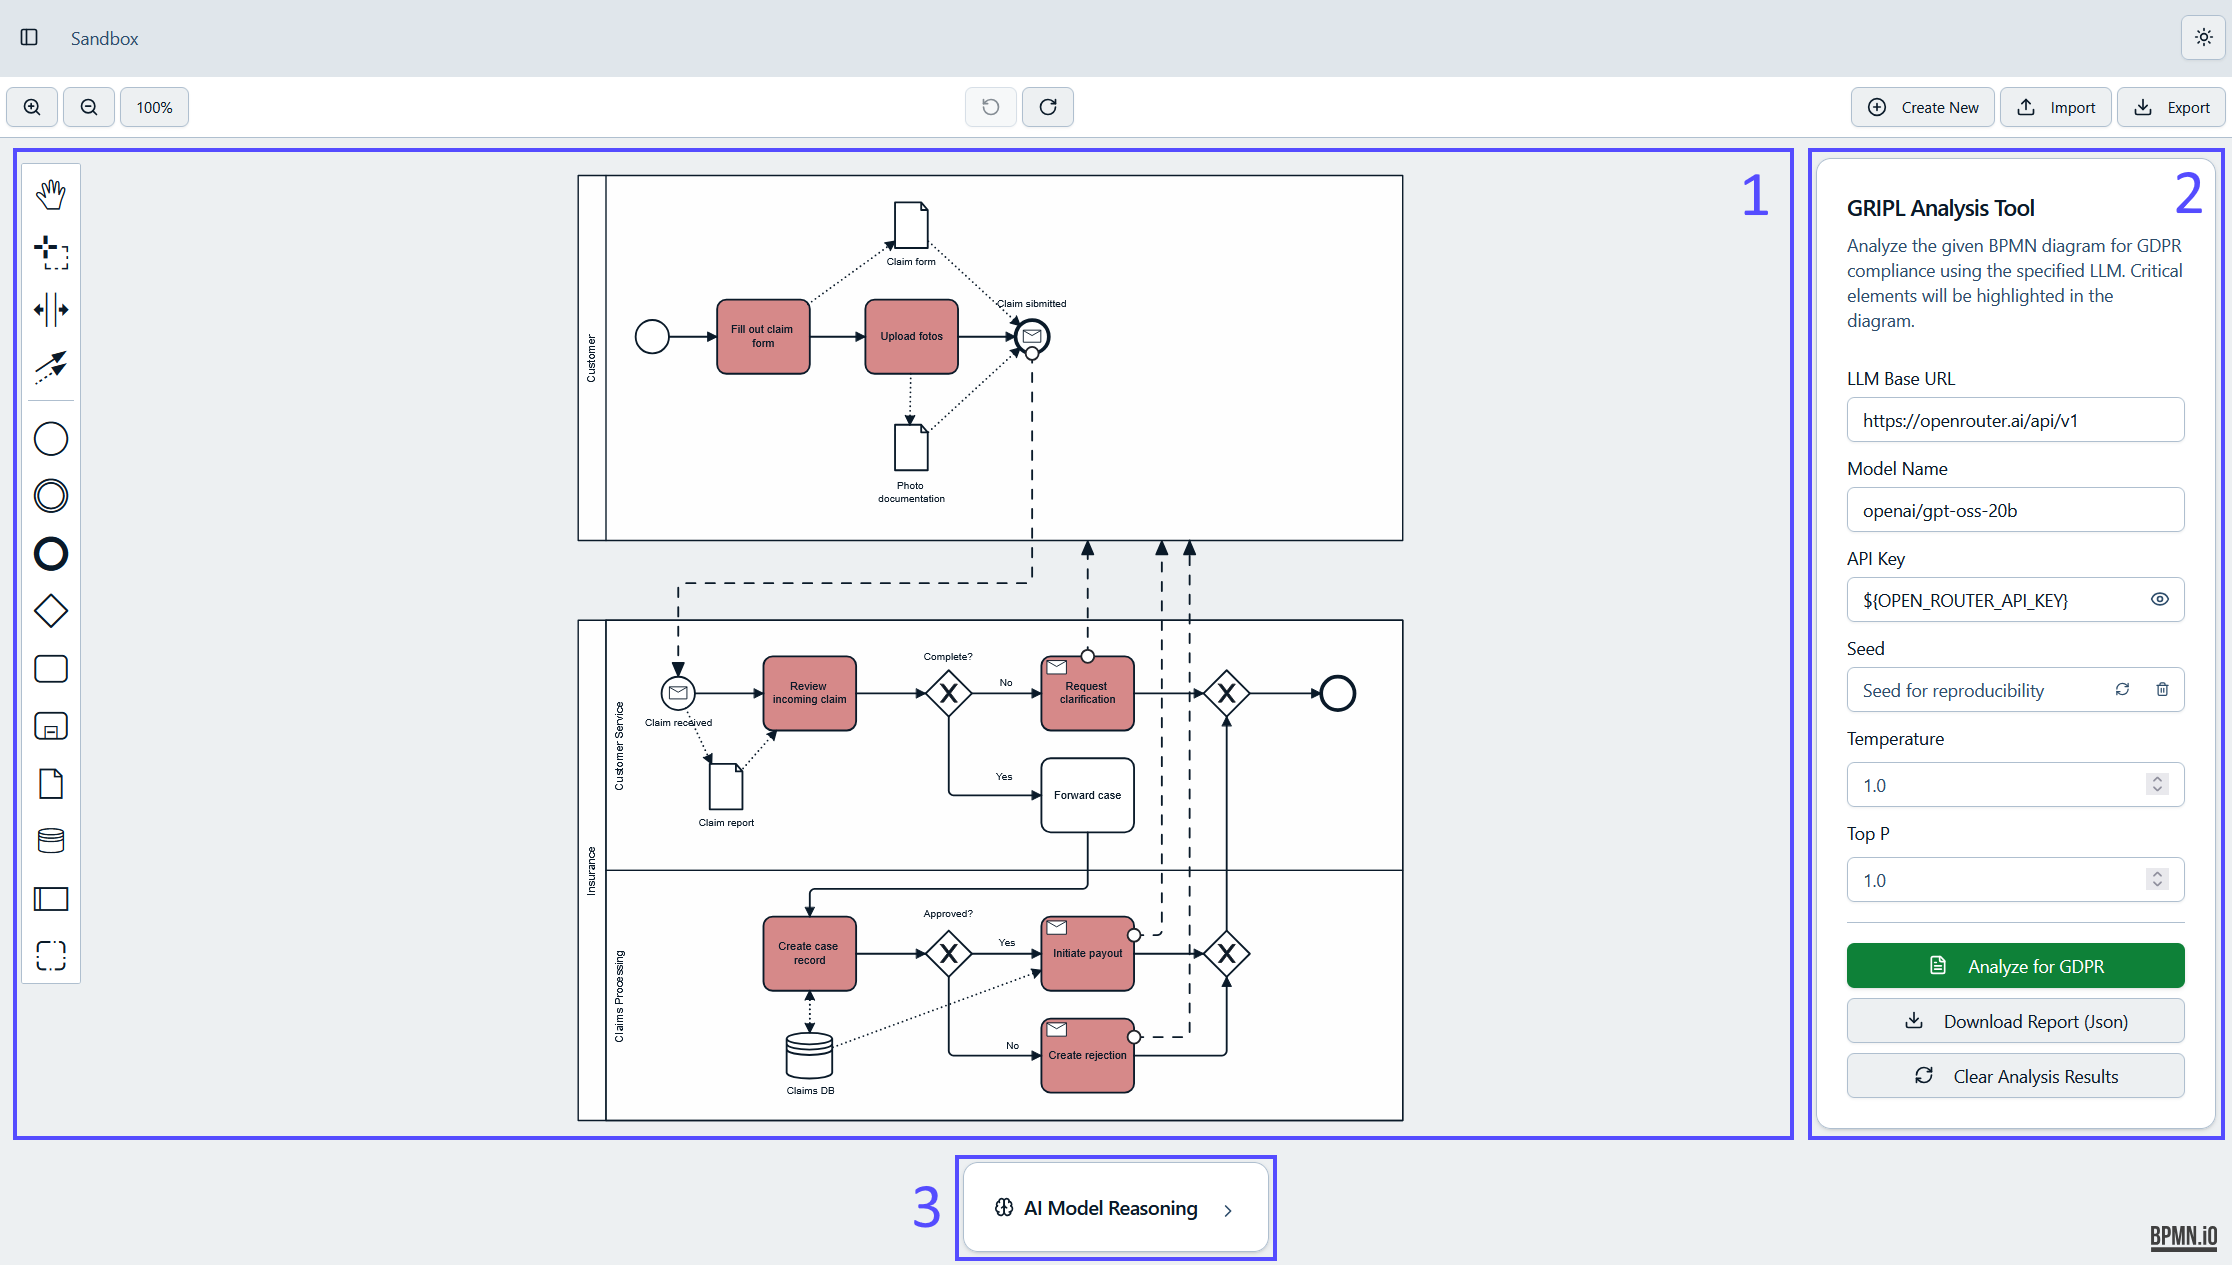
\includegraphics[width=\linewidth]{images/sandbox/sandbox-analyzed-model-annotated}
    \caption{Sandbox im Frontend mit hervorgehobenen kritischen Aktivitäten nach Analyse.}
    \label{fig:sandbox-frontend-analyzed-model}
\end{figure}

Die Webapp richtet sich primär an (1) Forschende und Studierende, die die Klassifizierungspipeline explorativ testen möchten, (2) Praktiker aus \ac{BPM} und Datenschutz (z.\,B. Prozessverantwortliche), die ein niedrigschwelliges Risiko-Screening einzelner Modelle benötigen, sowie (3) interessierte Dritte, die die in dieser Arbeit beschriebenen Ergebnisse reproduzieren möchten. Die Webapp schließt die Lücke zwischen der reinen API und typischen Modellierungswerkzeugen. Sie erlaubt ein Prototyping direkt am Prozessmodell, vermeidet lokale Installationshürden und dient als leichtgewichtige Demonstrationsoberfläche für Live-Analysen und Modellvergleiche.
Die in Abbildung~\ref{fig:sandbox-frontend-analyzed-model} markierten Bereiche strukturieren die Bedienoberfläche:

\begin{enumerate}
    \item \textbf{BPMN-Editor} (linke Hauptfläche): Vollwertiger Editor zum Modellieren, Importieren und Exportieren von \ac{BPMN}-Prozessen. Nach einer Analyse werden als kritisch eingestufte Aktivitäten unmittelbar im Diagramm farblich markiert.
    \item \textbf{Analyse-Panel} (rechte Seitenleiste): Konfiguration der \ac{LLM}-Eigenschaften und Start der Analyse. Neben Modell, Basis-URL und API-Schlüssel können u.\,a. Seed, \texttt{temperature} und \texttt{topP} gesetzt werden. Diese Parameter sind identisch zu den in Kapitel \ref{sec:api-design} beschriebenen \texttt{llmProps} und werden beim Starten der Analyse in die API-Anfrage überführt. Über Schaltflächen lassen sich die Ergebnisse als JSON herunterladen oder vorherige Markierungen löschen.
    \item \textbf{\ac{LLM}-Begründungen} (untere, aufklappbare Karte): Begründungen des \ac{LLM} zu jeder als kritisch erkannten Aktivität. Die Karte kann ein- und ausgeklappt werden. Eine geöffnete Ansicht ist in Abbildung~\ref{fig:sandbox-frontend-ai-reasoning} dargestellt.
\end{enumerate}

\begin{figure}[h]
    \centering
    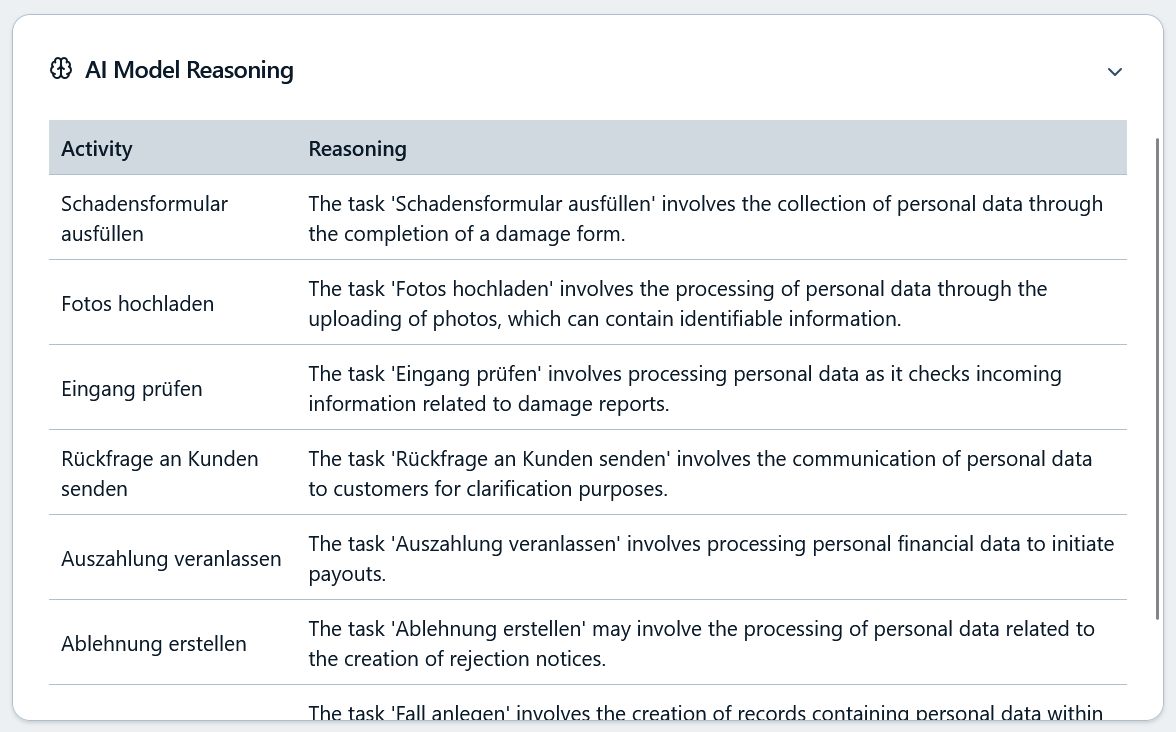
\includegraphics[width=.86\linewidth]{images/sandbox/sandbox-ai-reasoning}
    \caption{Exemplarische Begründungen der Klassifikation durch das LLM.}
    \label{fig:sandbox-frontend-ai-reasoning}
\end{figure}

Obwohl diese Arbeit auf Deutsch verfasst ist, verwendet die Webapp in der Benutzeroberfläche Englisch. Ebenso ist das \ac{LLM} in der Klassifikationspipeline über den System-Prompt auf Englisch eingestellt, sodass die generierten Antworten auf Englisch sind. Dies erhöht die Wiederverwendbarkeit für eine internationale Nutzerschaft. Die \ac{BPMN}-Modelle selbst können hingegen sowohl auf Deutsch als auch auf Englisch modelliert und analysiert werden.